\chapter{Introduction}

\section*{Exercise Solutions}

\begin{enumerate}
	\item Bounded by one plane: \textbf{half-space} \\
	Bounded by two planes: \textbf{infinite wedge} \\
	Bounded by three planes: \textbf{open ended infinite triangular prism} \\
	Bounded by four planes: \textbf{tetrahedron}
	
	\item Suppose figure \textit{A} is congruent to \textit{B} and figure \textit{B} is congruent to \textit{C}. Align \textit{A} and \textit{B} such that they completely coincide. We essentially have two names \textit{A} and \textit{B} for the same geometric figure. Now \textit{C} can be super-imposed onto \textit{B}, which is the same as \textit{A}. So \textit{C} coincides completely with \textit{A} hence \textit{C} and \textit{A} are congruent as well.
	
	\item If two different lines don't intersect they meet at zero points. Following the property mentioned in $\S4$ page 2, it is impossible for two distinct lines to coincide in two or more points. This implies that if two distinct lines intersect then they intersect at exactly point.
	
	\item If the line doesn't intersect a plane then they meet at zero points. Again following the property mentioned in $\S4$ page 2, if a line lies on a plane then it intersects with the plane at two or more points. This implies that if a line is NOT on the plane then it can intersect the plane at atmost one point.
		
	\item *
	
	\item Pick any two points on the plane. From $\S4$ we know that ``\textit{For every two points in space there is a unique line passing through these}''. Again as mentioned in $\S4$ we also know that ``\textit{If a straignt line passes through two points of a plane then this line lies on the plane}''. 
	
	\item Consider the following figure:
	
	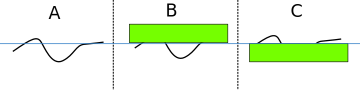
\includegraphics[scale=0.75]{chapters/ch00/images/07}
	
	If we align the straight edge along with the line. If line is perfectly straight then we should not see the ``bumps'' in figures B and C. If in one case the bumps were hidden underneath the ruler then flipping the ruler would reveal them.
	
	\item *
	
	\item For any point $p$ on a plane there are infinite other points on the same plane to form a pair. Let's call the second point $q$. From $\S4$ we recall that ``\textit{If a straight line passes through two points (p and q in this case) of a plane then this line lies on the plane}''. For each $p$ there exist infinite $q$ implying that infinite number of lines lying on the same plane as $p$ that pass through $p$.
	
	\item Cylinder, paper bent into an arc etc
	
	\item \underline{Infinite lines}: It is obvious to see
	
	\underline{Rays}: Move one of the rays such that the end points of both rays intersect. Now transform one of the rays such that it superimposes the other. Apply argument given for infinite lines above.
	
	\item Three steps are required:
	
	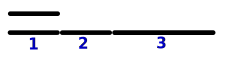
\includegraphics[scale=1.3]{chapters/ch00/images/12}
	
	\item Yes, it is unique. First find a sum of the given segments to obtain segment \textit{A}. Now find a segment on an infinite line a segment (not containing \textit{A}) that is congruent to \textit{A}. Let's call it \textit{B}. It is easy to show that \textit{B} is also the sum of given smaller segments because that's how we constructed \textit{B}, an identical copy of \textit{A}.
	
	\item yes, yes, yes
	
	\item Many examples. No, that is impossible.
	
	\item 
	
	\item 
	
	\item Couldn't understand the statement
	
	\item $\times$
	
\end{enumerate}